% !TEX program = xelatex
\documentclass{article}
\usepackage{/Users/Jay/LaTeX/cs}
\usepackage{/Users/Jay/LaTeX/matlab}
\usepackage{/Users/Jay/LaTeX/xeCJK}

\newcommand{\hmwkClass}{Digital Image Processing, Spring 2018}
\newcommand{\hmwkTitle}{Final Report}
\newcommand{\hmwkDueDate}{June 27, 2018}
\newcommand{\tb}{\textbf}

\begin{document}

\thispagestyle{empty}
\section*{\hmwkClass \\
    \normalsize{\hmwkTitle} \\
    \normalsize{DUE DATE: \hmwkDueDate}
}

\hfill{Team 23: \, R06945003 \, 林鈺盛 \, B03902129 \, 陳鵬宇} \\

\section*{Paper title}

Title: Fast Image Processing with Fully-Convolutional Networks \\
Conference: ICCV 2017 \\
Authors: Qifeng Chen, Jai Xu Intel Labs and Vladlen Koltun

\section*{Motivation}

Image processing can be used in everywhere. Like robotic navigation systems, traffic, healthcare, camera edge technology, etc. Faster image processing can save us tons of time. Learning how to accelerate the procedure of image processing is undoubtedly worthy.

\section*{Problem definition}

Use convolution neural network (CNN) to implement image processing methods mentioned in class.

\begin{itemize}
    \item Pencil Drawing
    \item Multi-scale Toning
    \item Photographic Style
    \item Nonlocal Dehazing
\end{itemize}

\section*{Algorithm}

\subsection*{Preliminaries}

Given:

\begin{itemize}
    \item \tb I: image in RGB space and
    \item $f$: operator, where \tb{I} and $f(\tb I)$ have the same resolution.
\end{itemize}

Our goal is:

\begin{itemize}
    \item to approximate $f$ with another operator $\hat f$, that is $f(\tb I) \approx \hat f(\tb I)$ for all images and
    \item to find a broadly applicable image processing operator.
\end{itemize}

There are three desirable criteria we want to meet with:

\begin{enumerate}
    \item Accuracy
    \item Speed
    \item Compactness
\end{enumerate}

\subsection*{Context Aggregation Networks (CAN)}

The primary architecture the paper used is \tb{multi-scale context aggregation network (CAN)}

Now let's describe the parameterization in detail.

The data lay out over layers: $\{\tb L^0, \dots, \tb L^d\}$.

\begin{itemize}
    \item Dimension of $\tb L^0$ (input) and $\tb L^d$ (output): $m \times n \times 3$.
    \item Dimension of $\tb L^s$ ($1 \le s \le d - 1$): $m \times n \times w$, where $w$ is the width (features) of each layer.
\end{itemize}

$\tb L^s$ can be computed from the previous layer $\tb L^{s - 1}$ as follows:

$$\tb L_i^s = \Phi\bigg( \Psi^s \bigg(b_i^s + \sum\limits_j \tb L_j^{s - 1} *_{r_s} \tb K_{i, j}^s \bigg)\bigg)$$

and $\Psi^s(x)$ is computed as follow:

$$\Psi^s(x) = \lambda_s x + \mu_s BN(x),$$

where $\lambda_s, \mu_s \in \mathbb R$ are learned scalar weights and $BN$ is the batch normalization operator. We'll keep training these two scalars for each iteration.

Specically, for image coordinates $x$:

$$(\textbf L_j^{s - 1} *_{r_s} \textbf K_{i,j}^s) (x) = \sum\limits_{a + r_s b = x} \textbf L_j^{s - 1}(a) \textbf K_{i,j}^s(b)$$

Performing dilated convolution needs to specify the kernel size, it looks like: \\

\begin{center}
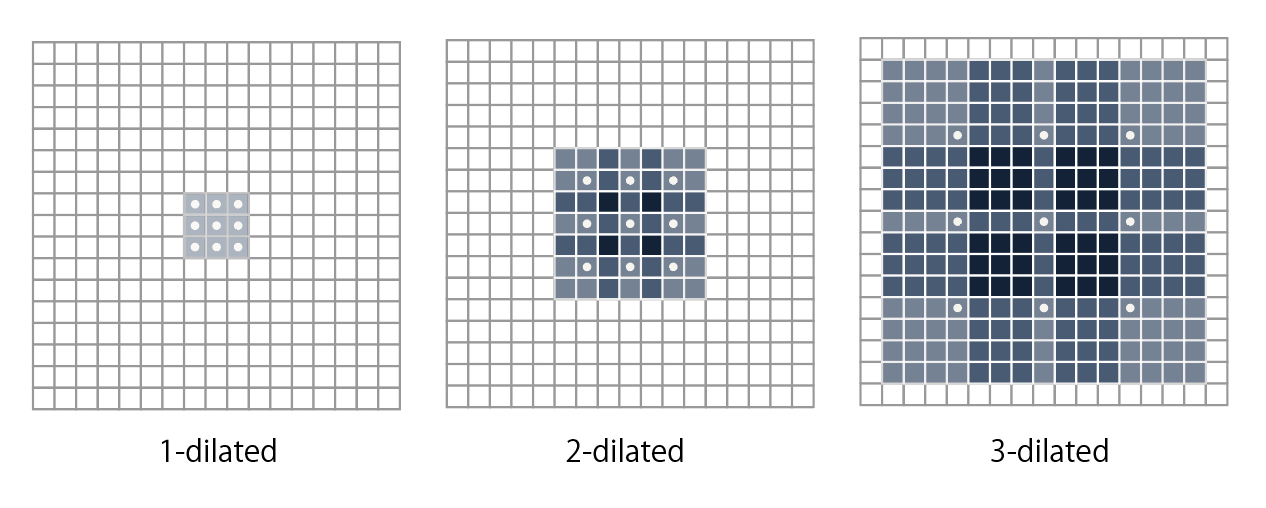
\includegraphics[width=0.8\textwidth]{img/dilated.png}
\end{center}

\subsection*{Batch Normalization}

\tb{Input:} Values of $x$ over a mini-batch: $\mathcal B = \{x_{1, \dots, m}\}$; Parameters to be learned: $\lambda, \beta$

\tb{Output:} $\{y_i = BN_{\gamma, \beta}(x_i)\}$

\begin{align*}
\mu_{\mathcal B}      & \leftarrow \frac{1}{m} \sum_{i = 1}^m x_i                                         & \text{mini-batch mean} \\
\sigma_{\mathcal B}^2 & \leftarrow \frac{1}{m} \sum_{i = 1}^m (x_i - \mu_{\mathcal B})^2                  & \text{mini-batch variance} \\
\hat x_i              & \leftarrow \frac{x_i - \mu_{\mathcal B}}{\sqrt{\sigma_{\mathcal B}^2 + \epsilon}} & \text{normalize} \\
y_i                   & \gamma \hat x_i + \beta \equiv BN_{\gamma, \beta}(x_i)                            & \text{scale and shift}
\end{align*}

\subsubsection*{Activation function (Leaky ReLU)}

\begin{itemize}
    \item Original: $\Phi(x) = \max(0.01x, x)$
    \item In this paper: $\Phi(x) = \max(0.2x, x)$
\end{itemize}

\subsection*{Training}

The network is trained on a set of input-output pairs that contain images before and after the application of original operator: $\mathcal D = \{\tb I_i, f(\tb I_i)\}$.

\begin{itemize}
    \item the parameters of the network are the kernel weights $\mathcal K = \{\tb K_{i, j}^s\}_{s, i, j}$ and
    \item the scalar biases $\mathcal B = \{b_i^s\}_{s, i}$.
\end{itemize}

These parameters are optimized to fit the action of the operator $f$ across all images in the training set.

We train with an image-space regression loss:

$$\ell(\mathcal K, \mathcal B) = \sum\limits_i \frac{1}{N_i} ||\hat f(\tb I_i; \mathcal K, \mathcal B) - f(\tb I_i)||^2,$$

where $N_i$ is the number of pixels in image $\tb I_i$.

\subsubsection*{Parameters}

\begin{itemize}
    \item epochs: 200
    \item batch size: 16
    \item optimizer: Adam(lr = 0.0003)
    \item loss function: MSE
\end{itemize}

\subsection*{Data spec}

\begin{itemize}
    \item MIT-Adobe 5k
    \item 2500/2500 training/test set
    \item 250 for validation
    \item Resize to $256 \times 256$ for training
\end{itemize}

\subsection*{Results}

\subsubsection*{Pencil Drawing}

\begin{center}
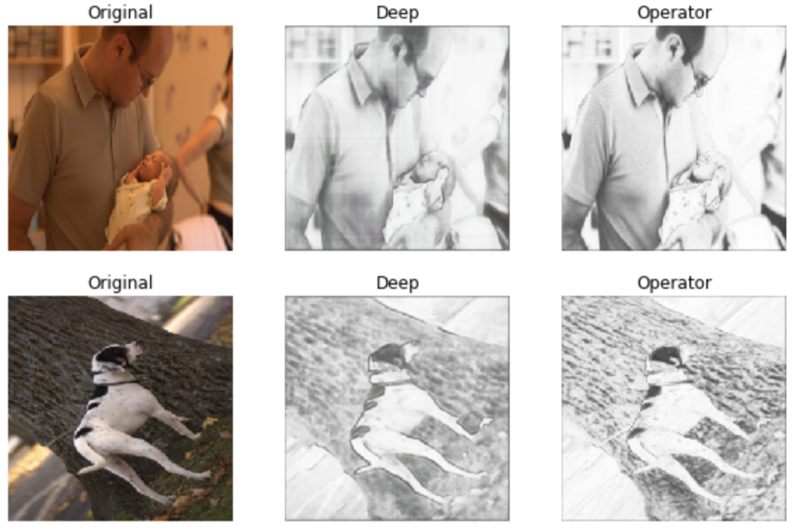
\includegraphics[width=0.8\textwidth]{img/1.png}
\end{center}

\subsubsection*{Multi-scale Toning}

\begin{center}
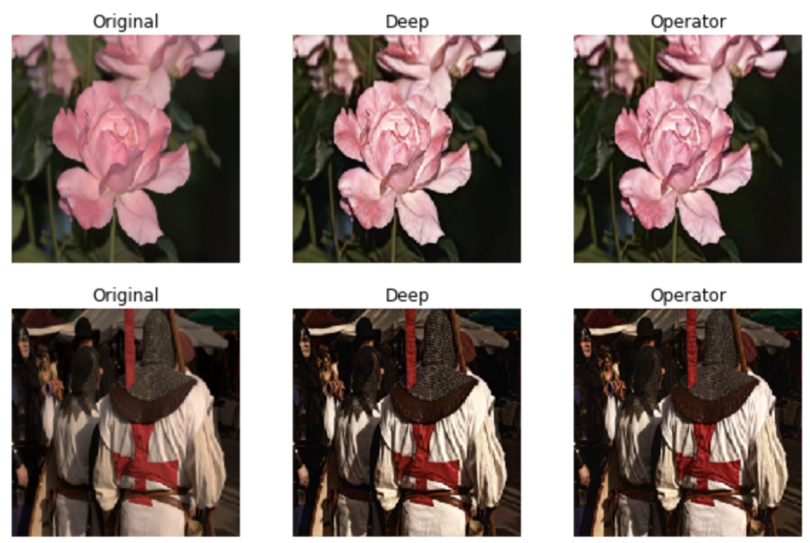
\includegraphics[width=0.8\textwidth]{img/2.png}
\end{center}

\subsubsection*{Photographic Style}

\begin{center}
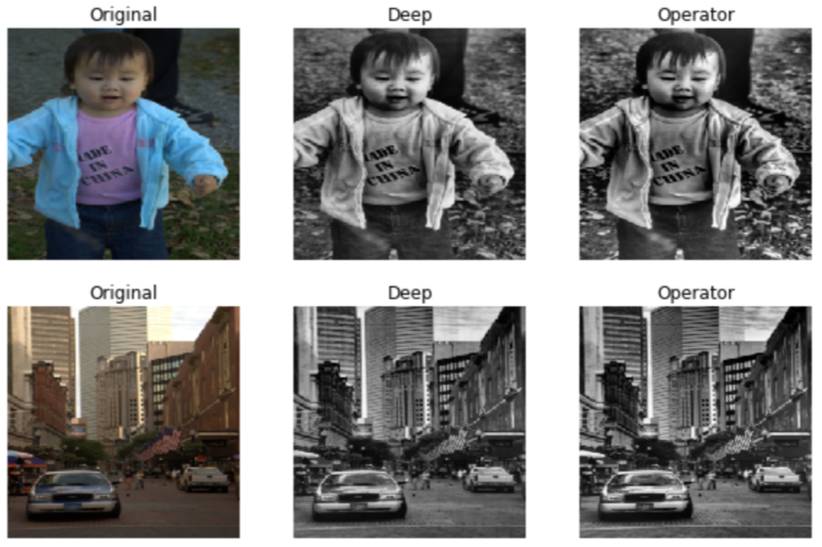
\includegraphics[width=0.8\textwidth]{img/3.png}
\end{center}

\subsubsection*{Nonlocal Dehazing}

\begin{center}
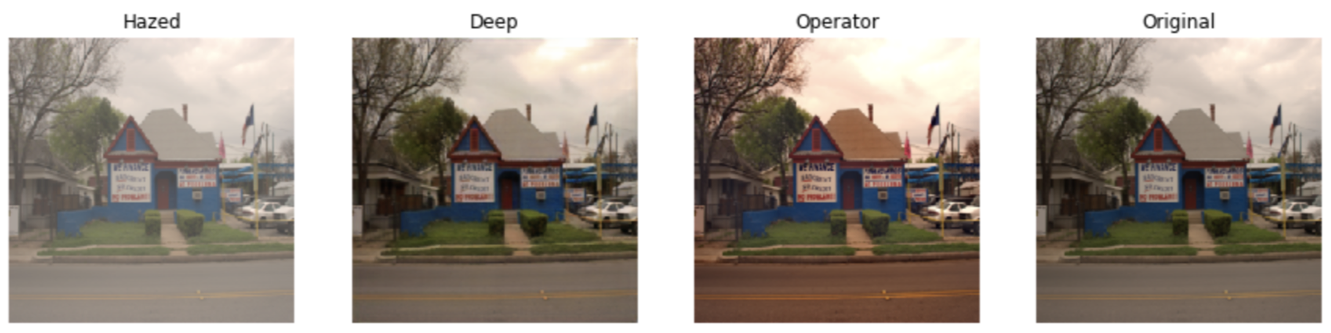
\includegraphics[width=0.8\textwidth]{img/4.png}
\end{center}

\begin{center}
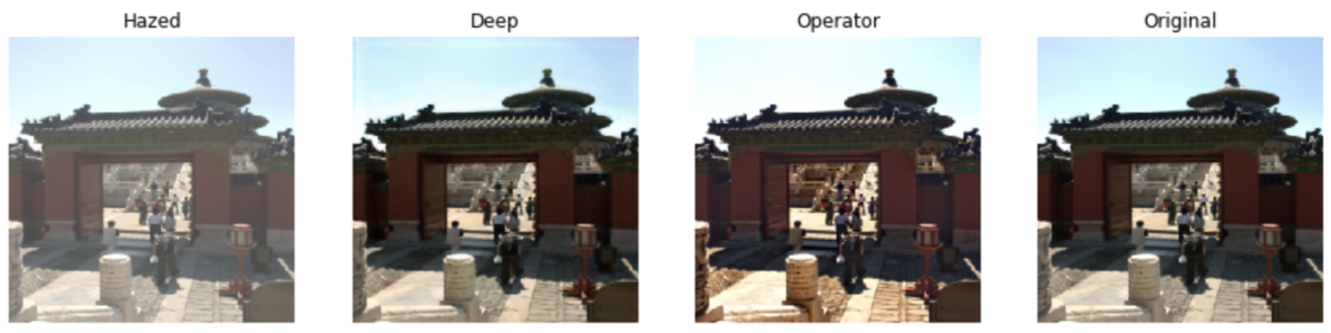
\includegraphics[width=0.8\textwidth]{img/5.png}
\end{center}

\subsection*{Discussion}

\begin{itemize}
    \item With sufficient computing resources, high-resolution images may be used for training
    \item Run time on predicting 2500 test images:
    \begin{itemize}
        \item Operator:2919 sec
        \item Deep model without GPU:1814 sec
        \item Deep model with GPU:70 sec
    \end{itemize}
    \item PSNR of Dehazing task:
    \begin{itemize}
        \item Deep model:29.32
        \item Operator:17.64
    \end{itemize}
\end{itemize}

\section*{Reference}

[1] \href{http://openaccess.thecvf.com/content_ICCV_2017/papers/Chen_Fast_Image_Processing_ICCV_2017_paper.pdf}{Fast Image Processing with Fully-Convolutional Networks}

[2] \href{https://arxiv.org/pdf/1511.07122.pdf}{Multi-scale context aggregation by dilated convolutions}

\end{document}